\chapter{Tổng quan}

%\section{Rendering of Eyes for Eye-Shape Registrationand Gaze Estimation}

%\section{EyeTab: Model-based gaze estimation on unmodified tablet computers}
Qua quá trình thực hiện luận văn Tôi đã tìm hiểu một số công trình nghiên cứu, bài báo khoa học nước ngoài, Tôi chưa tìm được báo cáo khoa học nào trong nước đi sâu vào đề tài nhóm đang hiện thực.

\section{Hiệu quả đánh máy bằng mắt với 9-hướng Gaze Estimation
 \cite{9direction}}
\textbf{Hướng tiếp cận}

Đầu tiên nhóm nguyên cứu tiến hành lấy mẫu (dataset) thực hiện chụp ảnh trực tiếp hay quay video người làm mẫu thực hiện 3 lần (3 top). Chia hướng nhìn thành 9 hướng và nhắm mắt. Tiến hành xử lý mẫu (dataset), phát hiện vị trí mắt trong ảnh, tiến hành cắt ảnh. Sau đó, xử lý ảnh trước khi đưa vào model hiện thực như: chỉnh độ sáng ảnh sử dụng HSV,... Tiếp theo, hiện thực kết quả với mô hình CNN (Lenet-5, Support Vector Machine (SMV),...)

\begin{center}
    \begin{figure}[h!]
    \begin{center}
     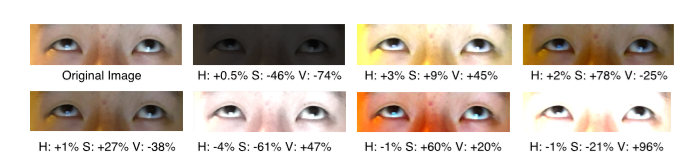
\includegraphics[scale=0.5]{img/yey.png}
    \end{center}
    \caption{Ảnh hưởng sau khi tăng chỉnh sáng}
    \label{refhinh15}
    \end{figure}
\end{center}

%\subsection{Mô hình thuật toán sử dụng}
\textbf{Mô hình thuật toán sử dụng}

\begin{center}
    \begin{figure}[h!]
    \begin{center}
     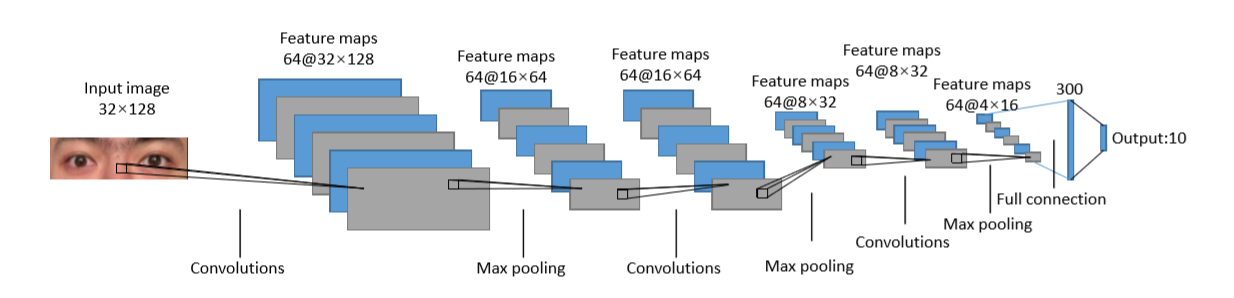
\includegraphics[scale=0.4]{img/yeycnn.png}
    \end{center}
    \caption{Ứng dụng mô hình CNN trong phát hiện hướng nhìn}
    \label{refhinh16}
    \end{figure}
\end{center}

Sử dụng các hình ảnh RGB với kích thước 32 x 128 pixel làm đầu vào mạng. Đối với lớp xoắn (convolution) đầu tiên, kích thước bộ lọc (filter) là 3x3 và bộ lọc (filter) dịch chuyển dọc theo ảnh và quét toàn bộ ảnh. Số lượng các bộ lọc là 64. Sau lớp xoắn, tiếp theo là ReLU và lớp tổng hợp tối đa (max pooling) thu được kích thước 64 x 16 x 64. Lặp lại hoạt động tương tự trên các lớp xoắn thứ hai và thứ ba. Lớp kết nối hoàn chỉnh (full connection) có 300 đơn vị ẩn và mỗi đơn vị có kết nối đến tất cả các bản đồ đặc trưng của lớp xoắn thứ ba. Đầu ra của mạng là mười loại (9 hướng mắt và nháy mắt), sử dụng chức năng softmax để tính toán tối ưu hóa.

\textbf{Kết quả đạt được}

Bảng thống kê dữ liệu thu được sau hai lần nguyên cứu lấy mẫu.

\begin{center}
    \begin{figure}[h!]
    \begin{center}
     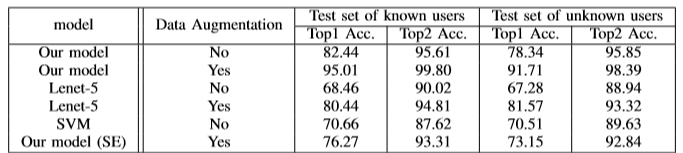
\includegraphics[scale=0.5]{img/table.png}
    \end{center}
    \caption{Bảng thống kê kết quả}
    \label{refhinh17}
    \end{figure}
\end{center}

Nhóm nguyên cứu đã quan sát thấy các hình ảnh ước lượng sai và phát hiện ra hướng sai, ước tính thường gần đúng hướng. Suy luận rằng có thể nguyên nhân ước lượng không chính xác, do người dùng định hướng sai cạnh của hai hướng liền kề. Nếu tính toán lỗi trên lần 2 (đợt lấy mẫu 2), tỷ lệ lỗi sẽ giảm xuống còn 0.2\%. Loại lỗi này có thể chấp nhận được vì khi sử dụng hệ thống để nhập từ (input words), người dùng luôn nhìn vào phần giữa của mọi hướng thay vì nhìn vào cạnh của hướng. Theo kết quả kiểm tra, mô hình với dữ liệu mắt đơn có tỷ lệ lỗi cao hơn. Từ tất cả các dữ liệu mắt người, ước tính sai, tìm thấy ba lý do sau đây: thứ nhất, dữ liệu mắt đơn nhạy cảm hơn với sự chuyển động nhẹ của đầu. Sự nghiêng đầu ảnh hưởng đến kết quả ước tính. Thứ hai, dưới độ phân giải thấp và điều kiện ánh sáng yếu, hình ảnh của mắt đơn có thể quá mờ để sử dụng ước lượng, ngay cả con người không thể nhận ra hướng. Thứ ba, mắt trái và phải không phải lúc nào cũng đồng bộ. Một số hình ảnh kết quả ước lượng của hai mắt là khác nhau nhưng cả hai đều hợp lý.

Để giải quyết những vấn đề tìm thấy, nhóm nguyên cứu đã thiết kế hệ thống bằng cách giải quyết cả vấn đề theo dõi mắt và các vấn đề nhập văn bản, phương pháp nhập văn bản dựa trên thị giác mà người dùng có thể nhập văn bản bằng chuyển động mắt và nhấp nháy, chọn các thanh điện thoại thông thường 9-key T9 bố trí bàn phím như giao diện. Một bộ dữ liệu quy mô lớn đã được thu thập bằng cách sử dụng một số thiết bị chụp và bao gồm các điều kiện ánh sáng khác nhau, địa điểm và thời gian. Sử dụng hình ảnh của cả hai mắt để tránh các vấn đề đồng bộ hóa hình ảnh mắt đơn, làm tăng độ chính xác ước lượng. Đối với các mục đích ứng dụng, xác định 9 hướng đi và học từ một mô hình CNN để đánh giá sự quan sát, có thể chính xác ước tính của người được biết đến (người tham gia lấy mẫu lần 2 trở lên) và người lạ (người tham gia lấy mẫu đầu tiên). Các phương pháp tăng dữ liệu được dùng cung cấp tính mạnh mẽ và tăng độ chính xác ước lượng. Phương pháp nhập văn bản này sử dụng các thiết bị có chi phí thấp, đơn giản hóa các bước hiệu chỉnh và lọc tiếng ồn do đường cong, nháy mắt tự nhiên và ước lượng sai lệch tạm thời trong suốt quá trình hoạt động, ngoài ra có thể chạy ở hai chế độ: chế độ ngoài màn hình và chế độ màn hình. Ở chế độ ngoài màn hình, người dùng có thể tự di chuyển và thiết bị cầm tay. Tốc độ nhập văn bản của chế độ màn hình có thể đạt 20 chữ trong một phút và tắt màn hình chế độ có thể đạt 18 chữ trong một phút với tỷ lệ lỗi thấp. Công việc trong tương lai của nhóm nghiên cứu này là giới thiệu mô hình ngôn ngữ và thêm các chức năng dự đoán và hoàn thành từ cho hệ thống hiện tại và đào tạo ước tính quan sát bất biến.
\section{Appearance-Based Gaze Estimation in the Wild \cite{appearance}}

\textbf{Hướng tiếp cận}

Hình ảnh đầu vào bước đầu được xử lý nhận diện khuôn mặt và điểm 6 điểm mốc (bao  gồm hai điểm của mỗi mắt và hai mốc điểm miệng). Sau đó dùng khuôn mặt 3D chung để ước tính các vị trí 3D của các điểm mốc đã được phát hiện và áp dụng công nghệ kỹ thuật chuẩn hóa không gian để cắt và biến dạng đứng đầu và hình ảnh mắt vào không gian đào tạo bình thường. Bước cuối cùng CNN  được đưa vào để học và đưa ra kết quả dự đoán.
\begin{center}
    \begin{figure}[h!]
    \begin{center}
     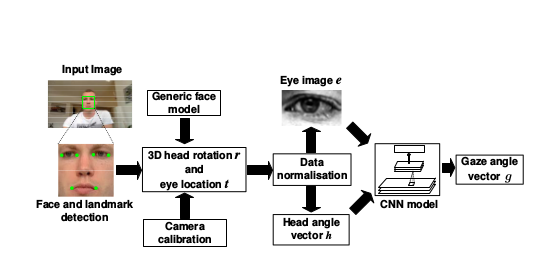
\includegraphics[scale=0.5]{img/h.png}
    \end{center}
    \caption{Xử lý đầu vào}
    \label{refhinh18}
    \end{figure}
\end{center}

\textbf{Mô hình thuật toán sử dụng}

Trong bài báo khoa học này tác giả sử dụng mạng LeNet bao gồm  một mạng tích chập (convolution) - hàm tổng hơp tối đa (max-pooling) - mạng tích chập - hàm tổng hợp tối đa - tầng kết nối đầy đủ (fully - connected). Lớp cuối cùng là một tuyến tính để đưa ra output cuối cùng. Đầu vào là hình ảnh màu xám có kích thước 60x36 pixels. Mỗi tích chập có kích thước feature 5x5 pixels, trong đó số feature của tầng thứ nhất là 20, tầng thứ 2 là 50. Đầu ra là hai góc nhìn, trái và phải.
\begin{center}
    \begin{figure}[h!]
    \begin{center}
     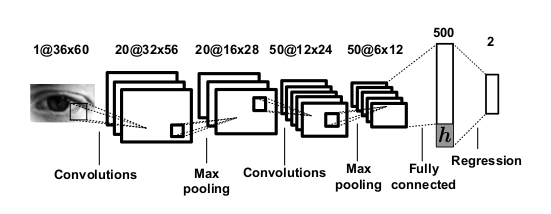
\includegraphics[scale=0.5]{img/conv.png}
    \end{center}
    \caption{Hình ảnh được đưa qua mạng học sâu để xử lý}
    \label{refhinh19}
    \end{figure}
\end{center}
\newpage
\textbf{Kết quả đạt được}

Bảng bên dưới là  sai số trung bình đạt được với môt số mô hình khác. Bao gồm Random Forests (RF), k-Nearest Neighbours(kNN), Adaptive Linear Regression (ALR), Support Vector Regression (SVR).
\begin{center}
    \begin{figure}[h!]
    \begin{center}
     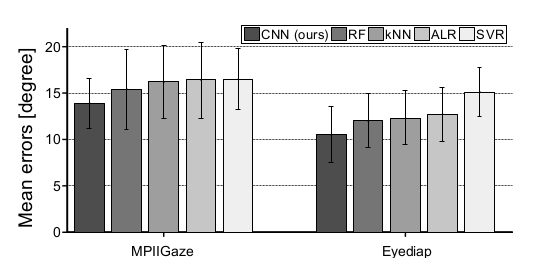
\includegraphics[scale=0.5]{img/2dataset.png}
    \end{center}
    \caption{Bảng thống kê kết quả}
    \label{refhinh20}
    \end{figure}
\end{center}
\section{Rendering of Eyes for Eye-Shape Registration and Gaze Estimation
\cite{eyeShapeRegistrationAndGazeEstimation}}
Nhóm nghiên cứu tạo ra một số lượng lớn hình ảnh thực tế của mắt bằng cách sử dụng mô hình vùng mắt động. Chúng được sử dụng làm dữ liệu đào tạo để đăng ký hình dạng mắt và ước tính dựa trên sự xuất hiện dựa trên sự xuất hiện.
\begin{center}
    \begin{figure}[h!]
    \begin{center}
     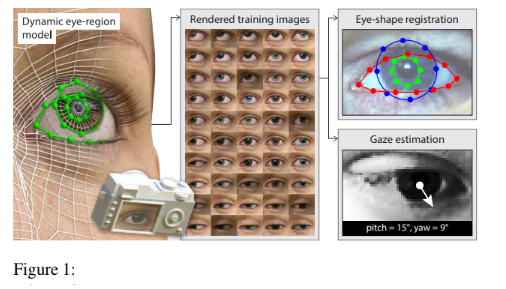
\includegraphics[scale=1]{img/photorealistic_images_of_eyes.png}
    \end{center}
    \caption{Chúng tôi tạo ra một số lượng lớn các hình ảnh photorealistic của mắt bằng cách sử dụng một mô hình vùng mắt động.}
    \label{refhinh20}
    \end{figure}
\end{center}
\textbf{Hướng tiếp cận}

(a) Quét hình ảnh 3D dày đặc (1,4 triệu đa giác (polygons))

(b) Được tái hiện lại thành dạng tối ưu cho hoạt ảnh (9,005 đa giác (polygons))

(c) Các chi tiết bề mặt da có độ phân giải cao được khôi phục bằng bản đồ dịch chuyển 

(d) Các điểm mốc mí mắt và mí mắt 3D được chú giải bằng tay 

(e) Hiển thị mẫu được hiển thị 
\begin{center}
    \begin{figure}[h!]
    \begin{center}
     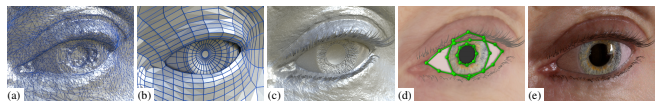
\includegraphics[scale=0.75]{img/An_overview_of_our_model_preparation_process.png}
    \end{center}
    \caption{Tổng quan về quá trình chuẩn bị mô hình.}
    \label{refhinh20}
    \end{figure}
\end{center}
Mô hình mắt nghiên cứu bao gồm các sclera, học sinh, mống mắt, và giác mạc (a) (the sclera, pupil, iris, and cornea) và có thể thể hiện sự thay đổi thực tế trong cả hai hình dạng (giãn nở đồng tử) và kết cấu (màu iris, tĩnh mạch scleral) (b).
\begin{center}
    \begin{figure}[h!]
    \begin{center}
     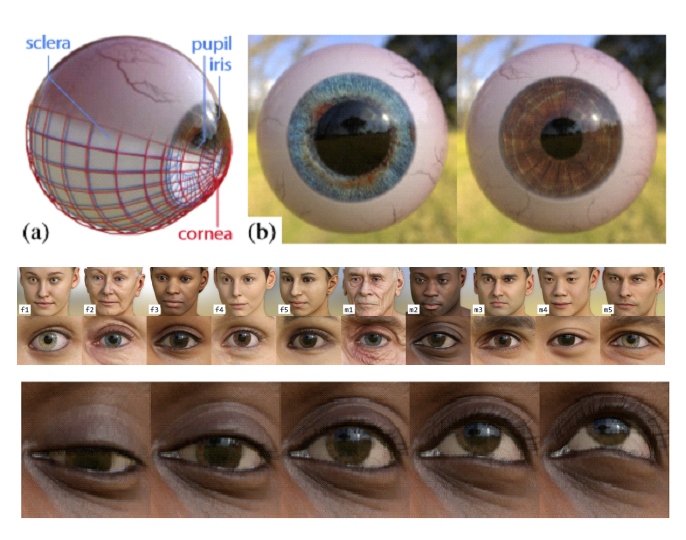
\includegraphics[scale=0.75]{img/Eye_model_and_3D_head_model.png}
    \end{center}
    \caption{Mô hình mắt và mô hình đầu (3D).}
    \label{refhinh20}
    \end{figure}
\end{center}

Máy ảnh được định vị để mô phỏng các thay đổi trong tư thế đầu (a). Tại vị trí này, chúng tôi hiển thị nhiều hình ảnh mắt cho các hướng nhìn khác nhau bằng cách đặt mô hình nhãn cầu (b):
\begin{center}
    \begin{figure}[h!]
    \begin{center}
     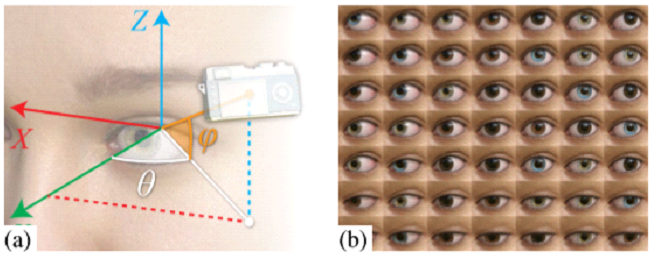
\includegraphics[scale=0.75]{img/Camera_position.png}
    \end{center}
    \caption{Vị trí máy ảnh.}
    \label{refhinh20}
    \end{figure}
\end{center}

Bốn bản đồ môi trường HDR, sử dụng cho ánh sáng thực tế: sáng / ngoài trời nhiều mây và sáng / tối trong nhà. Màu đỏ thể hiện điểm số tồi tệ nhất.

\begin{center}
    \begin{figure}[h!]
    \begin{center}
     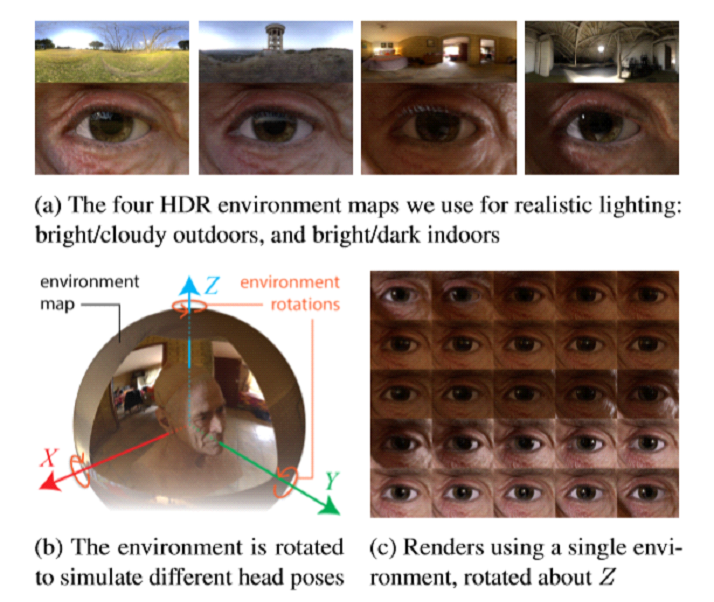
\includegraphics[scale=0.5]{img/Appearance_variation_from_lighting.png}
    \end{center}
    \caption{Sự biến đổi từ việc thay đổi ánh sáng được mô hình hóa với ảnh chụp có môi trường có phạm vi năng động cao.}
    \label{refhinh20}
    \end{figure}
\end{center}

\begin{center}
    \begin{figure}[h!]
    \begin{center}
     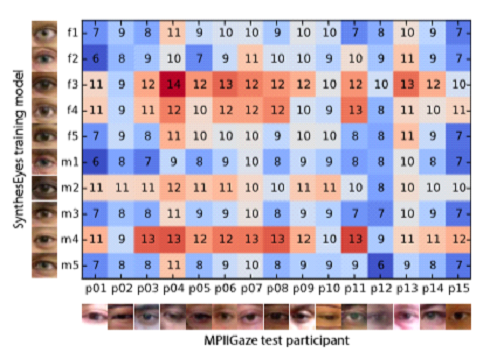
\includegraphics[scale=0.5]{img/Estimation_of_errors_on_MPIIGaze.png}
    \end{center}
    \caption{Ước lượng lỗi trên MPIIGaze}
    \label{refhinh20}
    \end{figure}
\end{center}
Nhóm nghiên cứu đã trình bày một phương pháp mới để tổng hợp những hình ảnh cận cảnh thực tế được dán nhãn hoàn hảo của mắt người. Một đường ống đồ họa máy tính sử dụng một bộ sưu tập các mô hình vùng mắt động thu được từ quét đầu để tạo ra các hình ảnh cho thấy phạm vi của các tư thế đầu, hướng nhìn và điều kiện chiếu sáng. Nhóm nghiên cứu đã chứng minh rằng phương pháp nghiên cứu hoạt động tốt hơn các phương pháp hiện đại để đăng ký hình dạng mắt và ước tính dựa trên sự xuất hiện dựa trên dữ liệu chéo trong tự nhiên. Những kết quả này hứa hẹn và nhấn mạnh tiềm năng quan trọng của các phương pháp tổng hợp học tập như vậy, đặc biệt là sự bứt phá với các phương pháp giám sát quy mô lớn gần đây.
\textbf{Kết quả đạt được}
Ví dụ về độ phù hợp (fits) với SynthesEyes eye-CLNF về hình ảnh trong tự nhiên (a) và hình ảnh webcam (b). Hai hàng hình ảnh trên cùng minh họa cho việc nhận dạng hình dạng mắt thành công, trong khi hàng dưới cùng minh họa các trường hợp thất bại, bao gồm các vệt chưa được tạo ra (tóc), các tư thế chưa được chỉnh sửa (mắt kín), kính và khởi tạo mô hình không chính xác.
\begin{center}
    \begin{figure}[h!]
    \begin{center}
     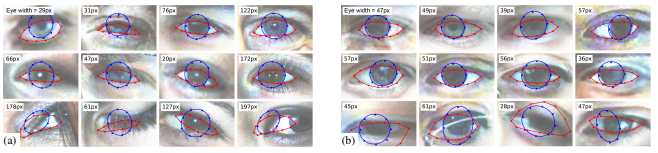
\includegraphics[scale=0.75]{img/Example_fits_of_our_SynthesEyes_eye_CLNF.png}
    \end{center}
    \caption{Ví dụ về độ phù hợp (fits) với SynthesEyes eye-CLNF}
    \label{refhinh20}
    \end{figure}
\end{center}
Trục x đại diện cho tập huấn luyện được sử dụng. Dấu chấm là các lỗi trung bình và đường màu đỏ thể hiện một giới hạn thấp hơn về mặt xác thực (số điểm xác thực chéo trong tập dữ liệu).

\begin{center}
    \begin{figure}[h!]
    \begin{center}
     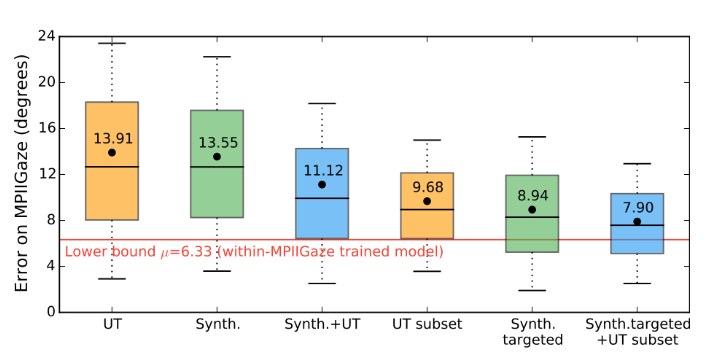
\includegraphics[scale=0.70]{img/Performance_chart_on_MPIIGaze.png}
    \end{center}
    \caption{Biểu đồ hiệu suất trên MPIIGaze}
    \label{refhinh15}
    \end{figure}
\end{center}

\section{Learning an appearance-based gaze estimator from one million synthesised images \cite{Learninganappearancebasedgazeestimator}}

\textbf{Hướng tiếp cận}

Nghiên cứu đã cung cấp một triệu hình ảnh thực tế về mắt bằng cách sử dụng mô hình vùng mắt được mô phỏng. Chúng được kết hợp với một hình ảnh đầu vào bằng cách sử dụng một phương pháp tiếp cận hàng xóm gần nhất (nearest-neighbor approach) để ước lượng cái nhìn. Mô hình quản lý này tìm ra các kết quả phù hợp ngay cả với các góc nhìn cực độ và ánh sáng chói từ kính.

\begin{center}
    \begin{figure}[h!]
    \begin{center}
     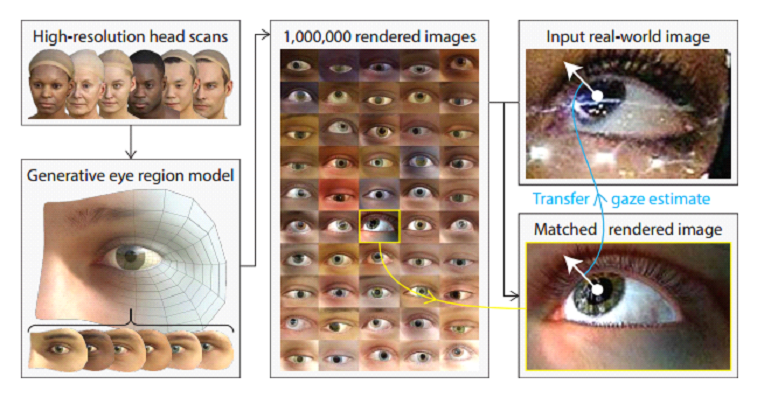
\includegraphics[scale=0.70]{img/Image_dataset_the_nearest_neighbor_approach.png}
    \end{center}
    \caption{Sử dụng phương pháp tiếp cận hàng xóm gần nhất(nearest-neighbor approach) để ước lượng cái nhìn.}
    \label{refhinh15}
    \end{figure}
\end{center}

Nhóm nghiên cứu trình bày về UnityEyes, một phương pháp mới để tổng hợp nhanh chóng số lượng lớn các hình ảnh vùng mắt thay đổi cho dữ liệu huấn luyện. Phương pháp nghiên cứu này: kết hợp một mô hình 3D sinh học mới lạ của vùng mắt người với khung thời gian thực. Mô hình vùng mắt có nguồn gốc từ quét khuôn mặt 3D có độ phân giải cao và sử dụng xấp xỉ thời gian thực cho các vật liệu và cấu trúc nhãn cầu phức tạp, cũng như các phương pháp hình học thủ tục lấy cảm hứng từ giải phẫu cho hoạt ảnh mí mắt. Tổng hợp hình ảnh bằng cách sử dụng trình kết xuất đồ họa và ánh sáng dựa trên hình ảnh thực tế và đa dạng điều kiện chiếu sáng. Những hình ảnh tổng hợp này có thể được khớp với hình ảnh đầu vào trong thế giới thực bằng cách sử dụng các phương pháp tiếp cận gần nhất để ước lượng ánh mắt. 

\begin{center}
    \begin{figure}[h!]
    \begin{center}
     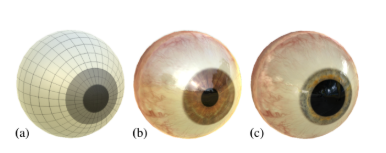
\includegraphics[scale=1]{img/Eyeball_mesh.png}
    \end{center}
    \caption{Hình ảnh về lưới mắt: (a) được hiển thị với các vật liệu dựa trên vật lý và các hiệu ứng khúc xạ, mô hình co rút đồng tử (b) và giãn nở (c).}
    \label{refhinh15}
    \end{figure}
\end{center}

\begin{center}
    \begin{figure}[h!]
    \begin{center}
     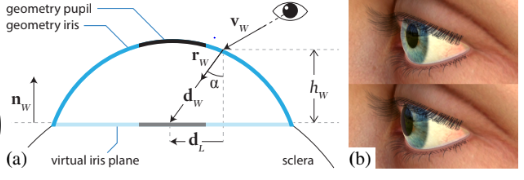
\includegraphics[scale=1]{img/Model_iris_refraction.png}
    \end{center}
    \caption{Mô hình khúc xạ iris bằng cách thay đổi kết cấu tra cứu: Một điểm ảnh được xem khúc xạ chính xác để hiển thị màu đen (tròng mắt) thay vì màu xanh (bề mặt hình học).}
    \label{refhinh15}
    \end{figure}
\end{center}

\begin{center}
    \begin{figure}[h!]
    \begin{center}
     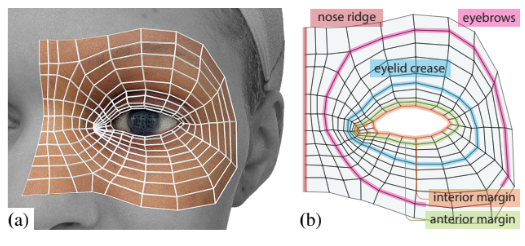
\includegraphics[scale=1]{img/Generative_eye_region_model.PNG}
    \end{center}
    \caption{Mô hình khởi tạo vùng mắt: (a) Cho thấy cấu trúc liên kết vùng mắt chung của chúng ta (229 đỉnh) trên một quét thô (khoảng 5M đỉnh). (b) Cho thấy cấu trúc liên kết trong không gian kết cấu uv với các vòng cạnh quan trọng được đánh dấu.}
    \label{refhinh15}
    \end{figure}
\end{center}

\textbf{Kết quả đạt được}

Nearest-neighbour pairs hiển thị hình ảnh tự nhiên (trên cùng) và phần kết của chúng tôi (dưới cùng) cùng với ánh mắt được ước tính (màu xanh lá cây).
Ba hàng đầu hiển thị ước tính chất lượng tốt, ngay cả dưới ánh sáng khó khăn (thiếu ánh sáng), độ phân giải thấp và góc nhìn cực đoan.
Hàng dưới cùng hiển thị các trường hợp lỗi từ biến thể chưa được sửa đổi, ví dụ: trang điểm và tóc.

\begin{center}
    \begin{figure}[h!]
    \begin{center}
     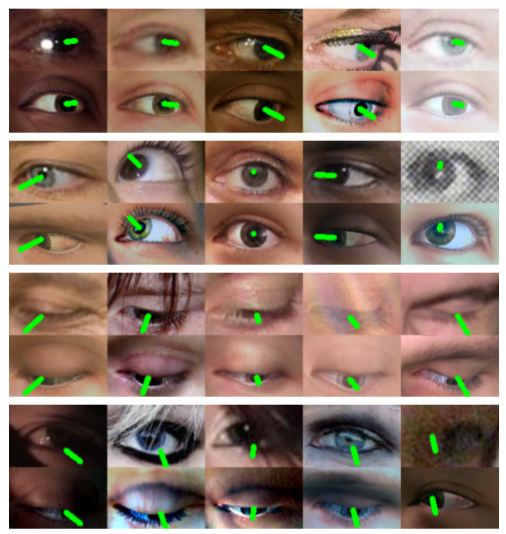
\includegraphics[scale=0.7]{img/The_result_of_Nearest_neighbour_pairs.png}
    \end{center}
    \caption{Kết quả của phương pháp tổng hợp những hình ảnh cận cảnh thực tế (Nearest-neighbour pairs) được dán nhãn hoàn hảo của mắt người }
    \label{refhinh15}
    \end{figure}
\end{center}

Lỗi pixel và điểm nhìn của phương pháp nearest-neighbor tương ứng với tập UnityEyes và MPIIGaze. Nhóm nguyên cứu đạt được lỗi thấp nhất ở 1.4 triệu hình ảnh.


\begin{center}
    \begin{figure}[h!]
    \begin{center}
     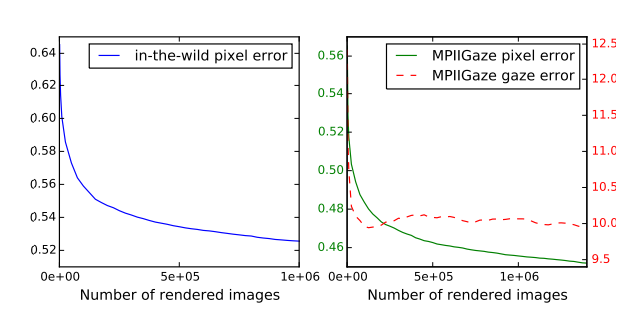
\includegraphics[scale=1]{img/Pixel_and_gaze_errors_for_nearest_neighbor.png}
    \end{center}
    \caption{Lỗi pixel và điểm nhìn của phương pháp nearest-neighbor tương ứng với tập UnityEyes và MPIIGaze. Nhóm nguyên cứu đạt được lỗi thấp nhất ở 1.4 triệu hình ảnh.}
    \label{refhinh15}
    \end{figure}
\end{center}


\newpage



